\documentclass[discrete.tex]{subfiles}

\begin{document}
  \section{Размещения, сочетания, перестановки без повторений}
  
  \begin{definition}
    Перестановка из n без повторений - упорядоченный набор из n неповторяющихся элементов, каждый из которых берется из диапазона $1:n$
    \[P_k = n!\]
  \end{definition}

  \begin{definition}
    Размещение - упорядоченный набор из k неповторяющихся элементов из диапазона $1:n$
    \[A_n^k = \dfrac{n!}{(n-k)!} = n (n-1)(n-k+1)\]
  \end{definition}

  \begin{definition}
    Сочетание - набор из k неповторяющихся элементов из диапазона $1:n$ (порядок не важен)
    \[C_n^k = \frac{A_n^k}{P_k} = \dfrac{n!}{(n-k)! k!}\]
  \end{definition}

  \begin{figure}[H]
      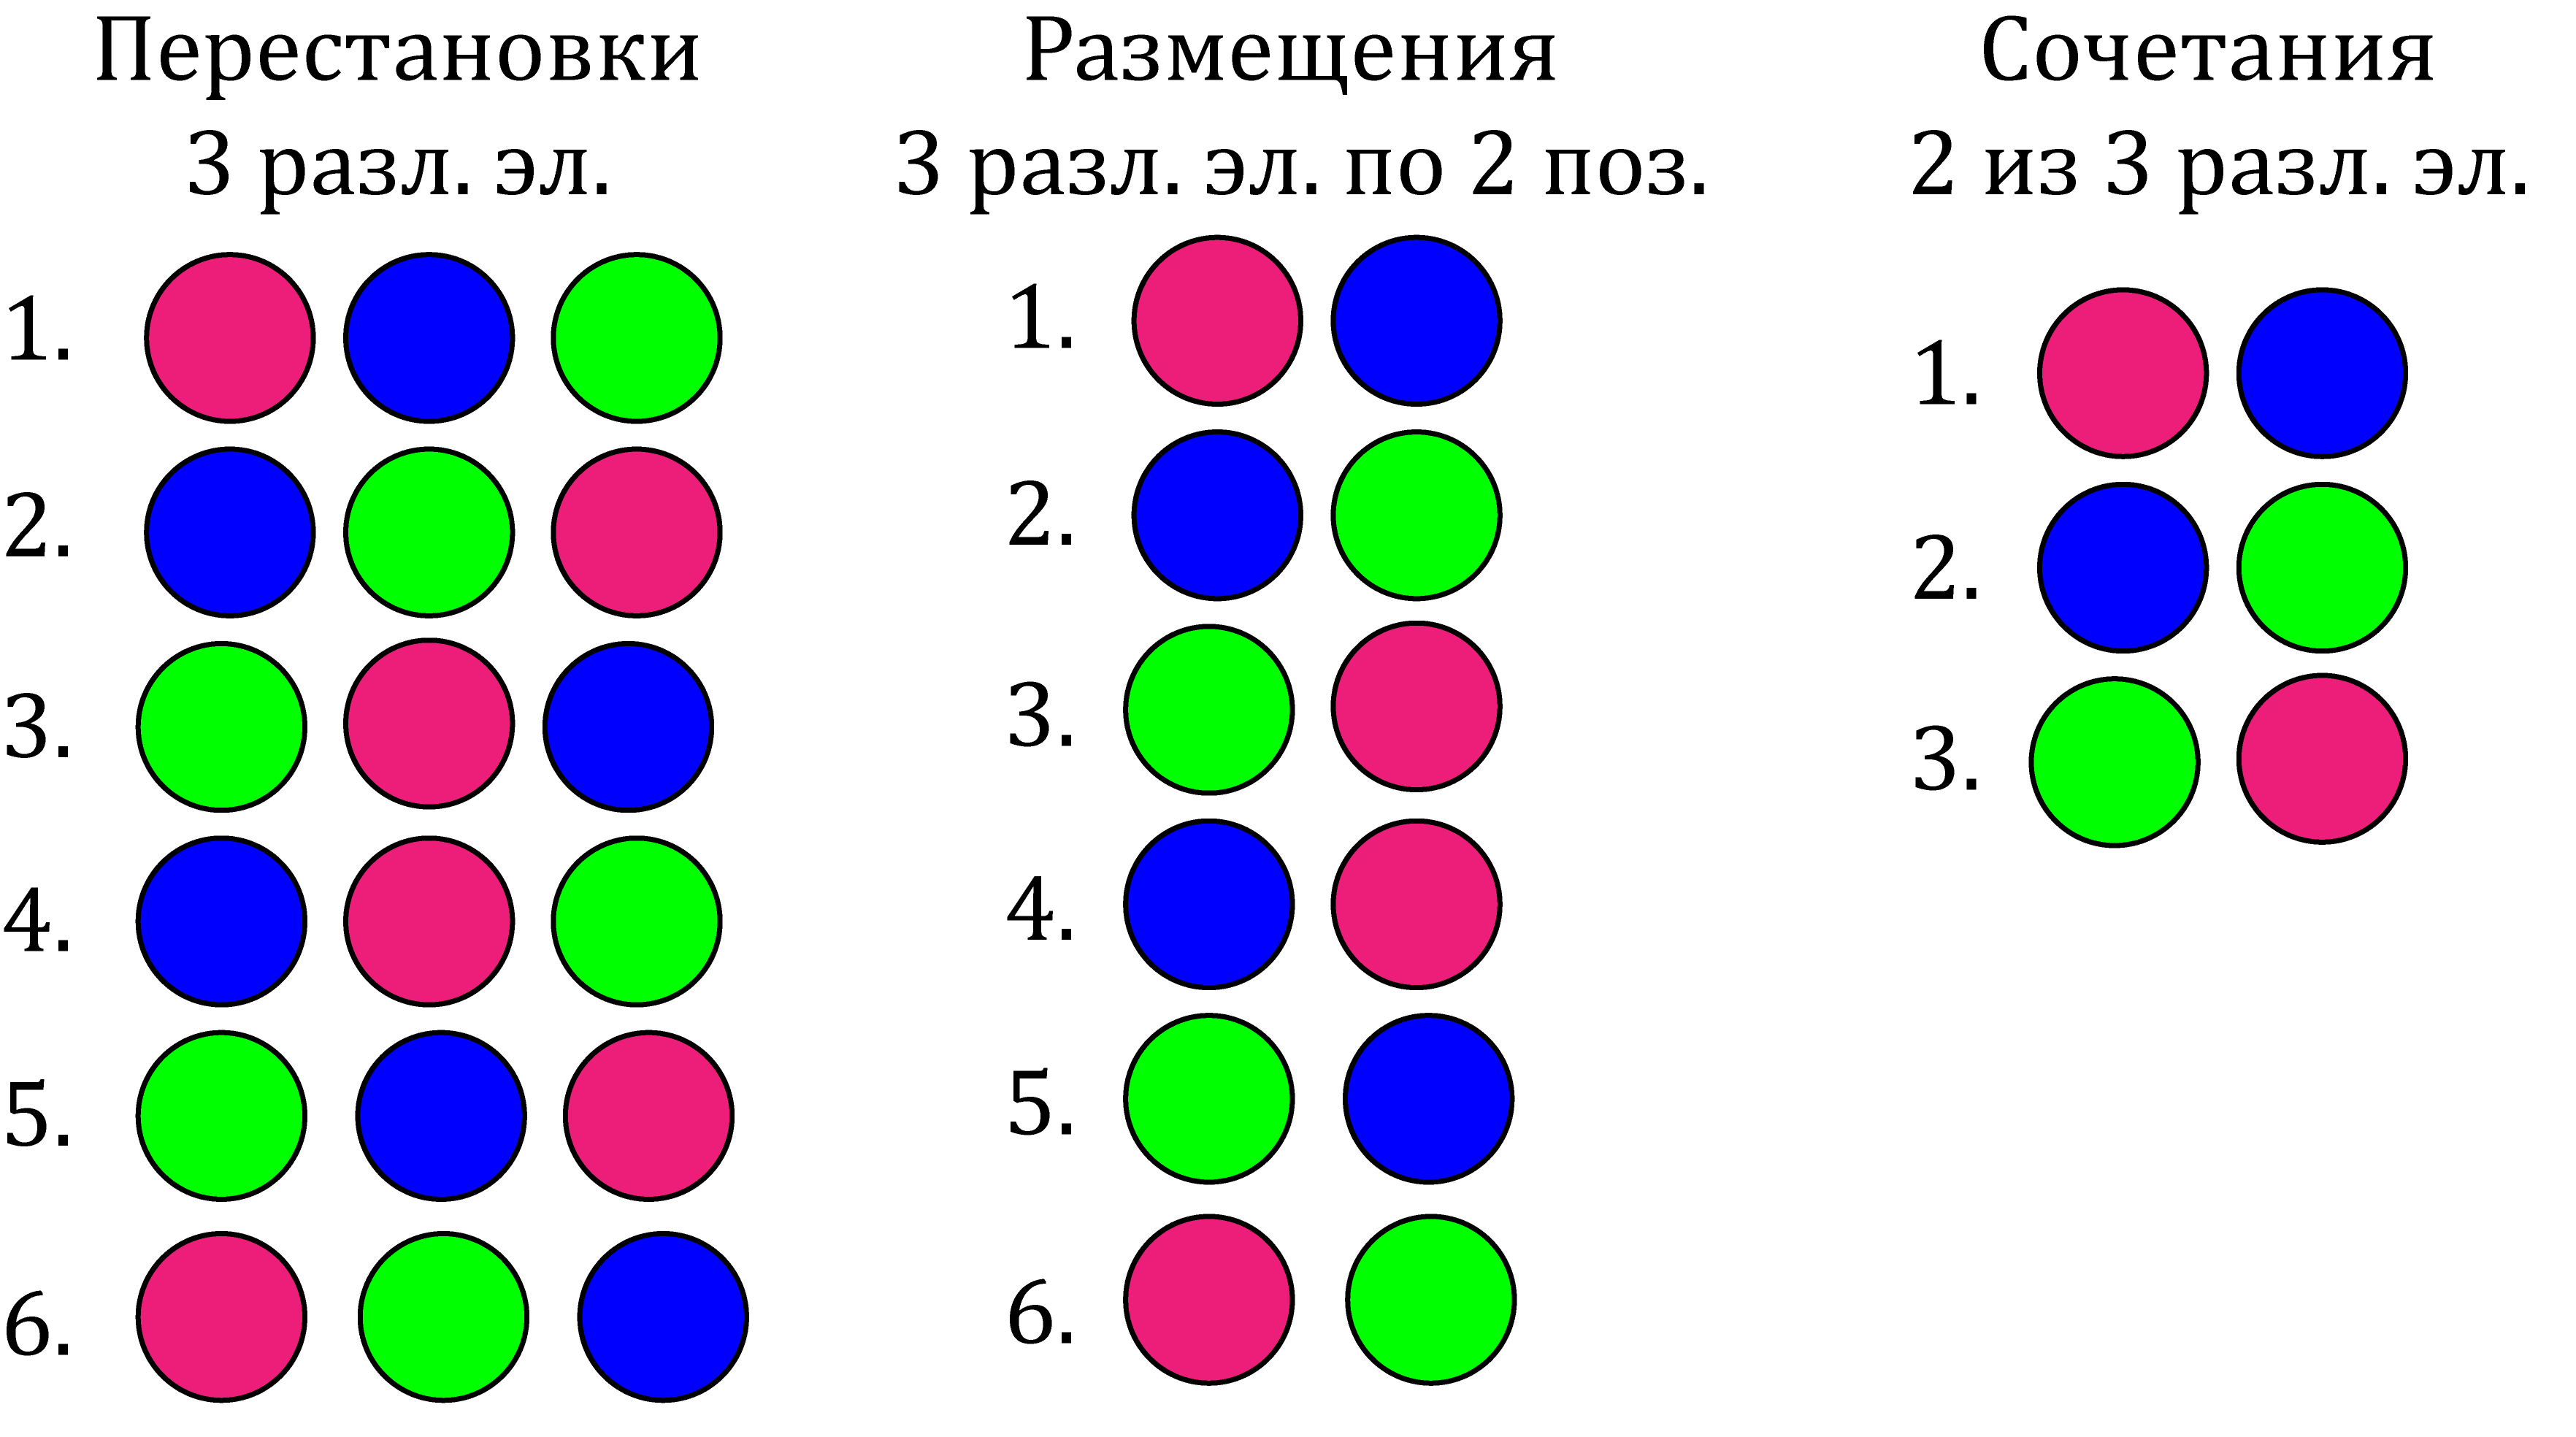
\includegraphics[width=10cm]{pics/5_1.png}
      \centering
  \end{figure}
\end{document}
